\documentclass[11pt,a4paper]{article}

\usepackage[margin=1in]{geometry}
\usepackage[T1]{fontenc}
\usepackage{lmodern}
\usepackage{amsmath,amssymb,amsthm}
\usepackage{mathtools}
\usepackage[protrusion=true,expansion=false]{microtype}
\usepackage{hyperref}
\usepackage{booktabs}
\usepackage{tabularx}
\usepackage{graphicx}
\usepackage{xcolor}
\usepackage{enumitem}
\usepackage{caption}
\usepackage{subcaption}
\usepackage{tikz}
\usepackage{pgfplots}
\pgfplotsset{compat=1.18}
\usepackage[numbers,sort&compress]{natbib}
\usepackage{url}

\hypersetup{
  pdftitle={The Constant in Front of sqrt(n): Measured Pollard Rho, ECC2K-130 Arithmetic, and Index Calculus over Prime Fields},
  pdfauthor={Anonymous},
  colorlinks=true,
  linkcolor=blue!50!black,
  citecolor=blue!50!black,
  urlcolor=blue!50!black,
}

\newtheorem{theorem}{Theorem}[section]
\newtheorem{lemma}[theorem]{Lemma}
\newtheorem{proposition}[theorem]{Proposition}
\theoremstyle{definition}
\newtheorem{definition}[theorem]{Definition}
\newtheorem{remark}[theorem]{Remark}

\newcommand{\FF}{\mathbb{F}}
\newcommand{\ZZ}{\mathbb{Z}}
\newcommand{\QQ}{\mathbb{Q}}
\newcommand{\Aut}{\operatorname{Aut}}
\newcommand{\Jac}{\operatorname{Jac}}
\newcommand{\ord}{\operatorname{ord}}
\newcommand{\HW}{\operatorname{HW}}
\renewcommand{\gcd}{\operatorname{gcd}}
\newcommand{\thislib}{\texttt{cryptanalysis}}
\newcommand{\sibling}{\texttt{crypto}}
% Footnote a number to a repository artefact. Paths without a repo prefix
% are in this library; paths prefixed crypto: are in the sibling.
\newcommand{\art}[1]{\footnote{\texttt{\detokenize{#1}}.}}

\title{The Constant in Front of $\sqrt{n}$: Measured Pollard Rho,
       ECC2K-130 Arithmetic, and Index Calculus over Prime Fields}
% Anonymized for double-blind submission.  Author block restored
% for camera-ready / preprint release; see paper/README.md.
\author{Anonymous}
\date{}

\begin{document}
\maketitle
\emergencystretch=2em

\begin{abstract}
This library measures discrete-logarithm algorithms in one unit
$S=\mathrm{ops}/\sqrt{n}$, against two boundaries: a counting floor
and a matched Pollard rho. On elliptic curves over prime fields and
over $\FF_{p^3}$ the method sits hundreds of times above rho at every
size that fits; the constant in front of $\sqrt{n}$ is the quantity
that moved, and it did not fall below one. The same unit prices a
multiplicative-group linear sieve that does cross rho near 56 bits, a
Koblitz GPU/FPGA iteration for ECC2K-130 whose pipe floor rules out
28 billion steps per second on one GPU, and a genus-3/4 Jacobian
positive control that behaves as the exponent law says.
\end{abstract}

\tableofcontents
\clearpage

\section{Introduction}
\label{sec:intro}

The discrete logarithm in a group of prime order $n$ has a generic
cost of $\Theta(\sqrt{n})$ group operations. Pollard's rho method
makes the leading constant about $\sqrt{\pi/2}\approx 1.25$ without
automorphisms and about $\sqrt{\pi/4}\approx 0.89$ with the negation
map~\cite{pollard1978,teske2001,bls2011}. Every subsequent algorithm
that claims to be faster is a claim about that constant, or about the
exponent. This paper measures both.

The work is a study library, not an attack on cryptographic sizes.
Field arithmetic is 64-bit Montgomery arithmetic; every problem the
library solves lives in a group of order below $2^{64}$. That bound is
deliberate. The purpose is to put every variant on one axis, with
every phase inside the cost, and to read off whether the constant in
front of $\sqrt{n}$ actually moved.

Three families are priced.

\paragraph{Pollard rho, and the square-root neighbours.}
Teske's $r$-adding walk, the negation map with Bernstein--Lange--Schwabe
cycle handling, one inversion per 256 additions, parameters chosen from
$n$. Baby-step giant-step, two grumpy giants and a baby, Pollard
kangaroo, Bernstein--Lange free precomputation, GLV folding, Cheon's
auxiliary-input attack, a CUDA kernel verified through a host emulator,
and a fleet protocol. The unit
\[
  S \;=\; \frac{\text{group operations}}{\sqrt{n}}
\]
makes rho a flat line. Everything else is a row.

\paragraph{ECC2K-130.}
The Certicom Koblitz challenge $y^2+xy=x^3+1$ over $\FF_{2^{131}}$,
group order $4\cdot r$ with $r$ a 129-bit prime, expected
$2^{60.9}$ iterations~\cite{bailey2009,certicom1997}. Optimal-normal-basis
arithmetic, three multiplier realisations, a golden C model, a bitsliced
client, a packed CUDA walk measured from $0.85$ to $14.64$~billion
iterations per second, a measured pipe floor that rules out $28$~B/s on
one GPU, a table walk declined at $16.56$ against a pre-declared $17.0$,
a per-GPU survey, a digit-serial FPGA core in this library ($362$
cycles/step, $7{,}941$ LUT4) and a companion engine measured on an AWS
F2 at $8.25$~G steps/s, and a live campaign at cutoff $32$ with
$2^{28.41}$ iterations per point, about $124$ million points, and no
collision.

\paragraph{Index calculus over prime fields.}
A Coppersmith--Odlyzko--Schroeppel linear sieve in $(\ZZ/p\ZZ)^*$ with
Lanczos and Hensel lifting, whose crossover with rho is near $56$~bits
and which we re-ran through $60$ and $62$~bits. Then the elliptic
negative: Semaev summation polynomials on $E(\FF_p)$ and residual walks
on $E(\FF_{p^3})$, priced phase by phase with fitted exponents, a
Joux--Vitse pair-only row, oracle rounds labelled as stage diagnostics,
and a genus-3/4 Jacobian positive control whose ratio to rho falls as
the exponent law predicts.

\subsection{What a number is allowed to mean}

A ratio to a boundary is the result; a constant that moved while the
ratio stayed flat is engineering; a headline count that fell while
total $S$ rose is relabelling; a number that changed because the
accounting did is a correction. Section~\ref{sec:method} states the
rule and works two cases. The residual-walk thread is the cautionary
one: its relation phase crosses rho near $2^{96}$ in isolation, while
the whole method never does, because the linear algebra it had left
out grows as $n^{0.68}$ against relations at $n^{1/3}$.

Wall-clock time is a practicality note. Operation counts survive
hardware. A run whose answer was not checked against a planted secret
is not a result. Companion CUDA rho over 256-bit primes, the ECC2K-95
kernel, and kangaroo code whose READMEs record that they have run only
through CPU emulation are kept out of headline claims; they appear as
cross-checks of the walk, not as device throughputs.

\subsection{Two repositories}
\label{sec:tworepos}

The measurements span two checkouts. This library (\thislib) is the
64-bit C11 reference: generic cyclic groups, the solvers of
Section~\ref{sec:rho}, the ECC2K-130 golden model and digit-serial FPGA
core, the imported packed GPU client held to that model, and the
$(\ZZ/p\ZZ)^*$ sieve. The sibling study library (\sibling), named from
\texttt{docs/ALGORITHMS.md}, is where the ECC2K-130 campaign, the GPU
ledger, the F2 FPGA engine, the residual-walk and hyperelliptic notes,
and the index-calculus scoreboard live. Paths in footnotes without a
prefix are in this library; paths beginning \texttt{crypto:} are in
the sibling. The paper covers both and says so here, once.

\subsection{What is not claimed}

No elliptic-curve index-calculus variant measured end to end sits
below matched rho. No one-addition-per-step walk on ECC2K-130 reaches
$28$~B/s on one GPU. No Modal SKU in the survey beats the RTX~PRO~6000
at the campaign recipe. The 256-bit CUDA rho of \texttt{crypto:gpu/ecc/}
and the ECC2K-95 kernel of \texttt{crypto:gpu/ecc2k/} are emulator-verified
walks, not device-throughput results. Extrapolations are marked as
such and carry the exponents they rest on.

\section{Method: boundary, unit, table, class}
\label{sec:method}

A thread that claims to improve an attack must express its progress as
a ratio to a boundary, reported in a single table whose rows are
variants and whose columns are one unit. A thread that cannot state
its boundary has not started; a thread whose ratio to the boundary is
flat has not progressed, however much its constants moved. The rule is
the reporting convention of the sibling study
library.\art{crypto:AGENTS.md}

\subsection{Two boundaries}

A \emph{boundary} is a quantity the method under study cannot cross,
derived rather than measured. A thread normally has one of each kind.

\begin{itemize}[leftmargin=1.2em,itemsep=0.3em]
\item A \emph{floor}: a lower bound from a counting or generic-group
  argument. For residual walks on $E(\FF_{p^3})$ a generic algorithm's
  expected relation yield from $P$ residuals is at most $\gamma P^2/2n$,
  so the count factor obeys $\kappa_{\mathrm{total}}\ge\sqrt{2(B+1)/\gamma}$.
  That floor moves only with the factor-base size $B$ and the
  automorphism order $\gamma$; it cannot be tuned
  away.\art{crypto:research/notes/index-calculus/RESEARCH_RESIDUAL_WALKS.md, §9.6}
\item A \emph{reference}: the cost of the best algorithm that already
  solves the same problem, measured in the same unit on the same
  instances. For the discrete logarithm that is Pollard rho, run on
  the same group, with the same operation accounting.
\end{itemize}

Both are written down \emph{before} optimising. A boundary chosen after
the fact is not a boundary.

\subsection{One table, one unit}

The unit used throughout is
\[
  S \;=\; \frac{\text{total operations}}{\sqrt{n}}.
\]
Rho is then a flat $S\approx 1.3$ at every size, and ``is this better
than rho'' is one column. Every cost the method incurs belongs in $S$:
precomputation, table setup, relation verification, linear algebra,
and any work an oracle does per call. Foreign units are converted with
a measured factor (for instance $63$ field multiplications per curve
addition on $\FF_{p^3}$) and the factor is recorded.

End-to-end speed is the measure of speed. $S$ is defined over the
whole method, cold, from setup to the recovered logarithm. A number
that prices only one phase --- the relation search, the decomposition
oracle, a single solver call, the linear algebra --- is a \emph{stage
diagnostic}, never a speed. ``Faster than rho'' means the method's $S$
column, with every phase inside it, sits below rho's, robustly, at
growing $n$. The only admissible speed ratio is
\[
  \mathrm{speedup}
  \;=\;
  \frac{\text{baseline total operations}}
       {\text{candidate total operations}}.
\]
A ratio taken over any smaller slice of the pipeline is labelled a
stage diagnostic and is not reported as a speedup. A row without a
verified answer is not a result.

\subsection{Four classes}

Every change is classified by what moved, not by how it felt to make.

\begin{center}
\small
\begin{tabular}{@{}llp{0.46\textwidth}@{}}
\toprule
class & what moved & what it means \\
\midrule
\textbf{advance} & ratio to the floor fell
  & the method does something a generic algorithm cannot \\
\textbf{engineering} & $S$ fell, ratio to the floor flat
  & legitimate, bounded, and not a finding \\
\textbf{relabelling} & headline count fell, $S$ rose
  & work moved somewhere the headline does not look \\
\textbf{accounting} & numbers changed, algorithm did not
  & a correction; say so and do not claim the gain \\
\bottomrule
\end{tabular}
\end{center}

All four are worth committing. Only the first is a result.

\subsection{Worked case: residual walks}
\label{sec:method-residual}

The residual-walk note is the reference implementation of the rule.
Section~9.6 of that note states the boundary and the numeric target
($\kappa_{\mathrm{total}}/\kappa_{\mathrm{floor}}<0.9$ on a hybrid at
fixed $B$, correct answer on every seed, zero relations failing
verification, zero trivial collisions counted as relations).
Section~9.7 freezes the baseline table. Section~10.6 classifies every
lever against the floor. Sections~11.5--11.6 are an engineering ledger
with the class of each step named. Section~11.7 prices the phase the
earlier rounds had skipped and corrects the conclusion they
implied.\art{crypto:research/notes/index-calculus/RESEARCH_RESIDUAL_WALKS.md}

The relabelling class is not hypothetical. In §10.5 a
triple-decomposition oracle cut the walked count from $16.3$ to
$0.15$, a hundredfold move in the number the thread had been tracking,
while total cost got $4.6\times$ worse: the count was not reduced, it
was paid for per residual instead of per step.

The skipped-phase mistake is the other half. Three rounds priced the
relation phase, quoted a crossover with rho at $2^{96}$, and left the
linear algebra unpriced. When it was measured it grew as $n^{0.68}$
against relations at $n^{1/3}$, so the method's cost bottoms out near
$200\times$ rho around $2^{50}$ and rises after. The $2^{96}$ was a
statement about one phase and had been read as a statement about the
method. That is the §5 mistake of the rule, named so that this paper
does not repeat it.

On $E(\FF_{p^3})$ at the sizes that fit, rho costs $S\approx 1.3$ and
every index-calculus variant built costs between $528\times$ and
$4{,}000\times$ that, with the asymptotically better variant crossing
rho only past $2^{230}$ (extrapolation, exponents in
Section~\ref{sec:ic-cubic}).

\subsection{Worked case: the ECC2K-130 pipe}
\label{sec:method-pipe}

The second worked case is a throughput floor rather than an operation
count. Any ECC2K-130 walk that keeps the rho collision structure
performs one affine addition per iteration. Affine addition with
batched inversion costs a fixed number of field products; a $131\times
131$ carry-less product is six \texttt{CLMAD}. The carry-less unit on
the RTX~PRO~6000 issues at about $1.6$ lane-operations per SM-clock.
Those two facts write a floor in billions of iterations per second
before any kernel is tuned: $28$~B/s needs $\le 25.4$--$26.9$
\texttt{CLMAD} per update including squarings and inversion, and the
arithmetic floor is already $28.9$ even with squarings moved
elsewhere.\art{crypto:ecc2k130/ITERATION-FUNCTION.md, §1}

Every subsequent GPU row is engineering against that floor. The table
walk of Section~\ref{sec:tablewalk} declared $17.0$~B/s as its own
target before the build; it measured $16.56$ and was declined. That is
the rule working in the other direction: a pre-declared numeric
condition that a later run either meets or does not.

\subsection{What does not count}

A ratio improved by moving the boundary, changing the unit, or
dropping a cost from the budget; a count lowered without the total
falling; an extrapolation presented as a measurement; a run whose
answer was not checked against the planted secret; wall-clock time as
the headline. Extrapolate freely, and mark it as extrapolation with
the exponents it rests on. Fit exponents over at least four sizes and
report the fit next to the prediction.

\section{Pollard rho}
\label{sec:rho}

Pollard rho is the reference. This section records the walk this
library actually runs, the constants it measures, and the GPU and
fleet machinery that parallelise it without changing $S$.

\subsection{The walk}
\label{sec:rho-walk}

The solver is Teske's $r$-adding walk~\cite{teske2001}. Multipliers
$M_i=\alpha_i G+\beta_i H$ are drawn once per job; the state is
$(Y,a,b)$ with $Y=aG+bH$; a step is $Y\leftarrow Y+M_{\mathrm{idx}(Y)}$.
Distinguished points --- hashes with \texttt{dp\_bits} trailing zero
bits --- are stored with their $(a,b)$ in a shared table (van
Oorschot--Wiener~\cite{vanoorschot1999}). A second arrival with a
different $(a,b)$ gives $(b-b')x=a'-a\pmod n$. For composite $n$ the
congruence is solved by gcd and every candidate is
verified.\art{src/rho.c}\art{docs/ALGORITHMS.md, ``Pollard rho''}

$r$, the number of walks per thread $W$, and \texttt{dp\_bits} are
chosen automatically from $n$ and the thread count so that neither the
multiplier table nor the walk start-ups (each about $3\log_2 n$
operations) exceed a small fraction of $\sqrt{n}$, and so that the
expected number of distinguished points is about 32 per walk, bounded
above at $2^{24}$ table entries. Walks that run $24\cdot
2^{\texttt{dp\_bits}}$ steps without a distinguished point are
restarted.

Threads run batches of $W$ walks; each batch step is one
\texttt{ca\_group\_batch\_op}, Montgomery's simultaneous
inversion~\cite{montgomery1987}. On one core an affine curve addition
costs $232.2$~ns with a private inversion and $21.8$~ns in batches of
$256$ ($45.88$~Mops/s), a $10.6\times$
saving.\art{docs/BENCHMARKS.md, ``Raw group operation throughput''} A
$61$-bit $(\ZZ/p\ZZ)^*$ Montgomery multiply is $5.9$~ns
($169.4$~Mops/s) on the same host.

\subsection{Negation map and fruitless cycles}

On elliptic curves every point is replaced by the canonical member of
$\{Y,-Y\}$ (the one with the smaller Montgomery $y$), negating $(a,b)$
when needed. The search space shrinks by $2$ and the expected cost by
$\sqrt{2}$. The walk on classes is well defined because $\mathrm{idx}$
is evaluated on the canonical form.

Fruitless cycles are handled as in Bernstein--Lange--Schwabe~\cite{bls2011}:
\begin{itemize}[leftmargin=1.2em]
\item \emph{2-cycles.} The look-ahead rule ``if $\mathrm{idx}(Y+M_i)=i$
  use $M_{i+1}$ instead'' (iterated) keeps the walk a deterministic
  function of $Y$ and reduces the 2-cycle rate from $1/(2r)$ to about
  $1/(2r)^2$.
\item \emph{Longer cycles.} A sliding window compares each new point
  with a point saved every 64 steps. On a hit the cycle is traversed
  once, its minimum (by hash) found, and the walk escapes
  deterministically to $2\cdot\min$. Because the escape depends only
  on the cycle, two walks that merged inside a cycle stay merged.
\end{itemize}
With the negation map, $r$ is allowed to grow to $1024$; without it
the default is $32$.

\subsection{Measured $S$}
\label{sec:rho-S}

Table~\ref{tab:rho-s} is the whole-group table of
\texttt{docs/BENCHMARKS.md}: prime-order $(\ZZ/p\ZZ)^*$ subgroups of
safe primes and prime-order curves, five instances per row, $S$
counting every thread's operations. With five repetitions the rho and
kangaroo rows carry about $\pm 25\%$ statistical noise (the standard
deviation of one run is about half its mean), so the honest summary is
that rho, kangaroo and grumpy giants all sit at $S\sim 1.2$--$1.8$,
BSGS at $1.5$, as theory says.\art{docs/BENCHMARKS.md, ``Whole-group discrete logarithm''}

\begin{table}[t]
\centering
\small
\caption{Whole-group discrete logarithm, $S=\mathrm{ops}/\sqrt{n}$,
  5 instances per row, 4 threads for \texttt{rho-T}. From
  \texttt{ca\_bench generic --threads 4}.}
\label{tab:rho-s}
\begin{tabular}{@{}lrrrrr@{}}
\toprule
grp & bits & BSGS & rho-1 & kangaroo & grumpy \\
\midrule
$\ZZ_p^*$ & 24 & 1.496 & 2.066 & 1.751 & 1.242 \\
$E(\FF_p)$ & 24 & 1.496 & 1.603 & 1.886 & 1.211 \\
$\ZZ_p^*$ & 32 & 1.575 & 1.256 & 1.412 & 1.365 \\
$E(\FF_p)$ & 32 & 1.575 & 0.791 & 2.174 & 1.514 \\
$\ZZ_p^*$ & 36 & 1.441 & 1.563 & 1.691 & 1.351 \\
$E(\FF_p)$ & 36 & 1.441 & 1.283 & 1.768 & 1.413 \\
$\ZZ_p^*$ & 40 & 1.573 & 0.887 & 1.795 & 1.393 \\
$E(\FF_p)$ & 40 & 1.573 & 1.713 & 1.220 & 1.251 \\
\bottomrule
\end{tabular}
\end{table}

One-thread rho on $32$-bit $\ZZ_p^*$ is $S=1.256$; on curves with the
negation map the 24--40-bit span is $0.791$--$1.713$. The wall-clock
column of the source table (not reproduced) shows the structural
facts: table-based methods slow down per operation as the table grows,
rho stays at $40$--$100$~Mops/s in $\ZZ_p^*$ and $10$--$20$~Mops/s on
curves, and kangaroo is the fastest per operation because it stores
almost nothing.

Interval logarithms of width $2^w$ inside a $\sim 2^{60}$ ($\ZZ_p^*$)
or $\sim 2^{56}$ (curve) group sit at $S=\mathrm{ops}/\sqrt{w}$ of
$1.5$--$2.8$. A separate 400-instance run of grumpy giants gives
$S=1.78$ for intervals and $1.18$ for whole groups; the five-instance
rows scatter around those
values.\art{docs/ALGORITHMS.md, ``Two grumpy giants and a baby''}

\subsection{Fitted exponents}

$S$ assumes the exponent is $1/2$. The library also measures it.
\texttt{ca\_bench complexity --bits 20,24,28,32,36 --reps 5} fits
$\mathrm{cost}\sim C\cdot N^{\alpha}$ in log-log space and reports
$\alpha$ next to the theoretical exponent
(Table~\ref{tab:exponents}).\art{docs/BENCHMARKS.md, ``Measured time complexity''}

\begin{table}[t]
\centering
\small
\caption{Fitted exponents, five sizes, five repetitions. The last
  column is $\mathrm{mean}(\mathrm{cost}/N^{\mathrm{theory}})$, the
  familiar $S$, meaningful because the fitted $\alpha$ confirms the
  exponent.}
\label{tab:exponents}
\begin{tabular}{@{}llrrr@{}}
\toprule
algorithm & theory & $\alpha$ & $R^2$ & const \\
\midrule
BSGS ($\ZZ_p^*$) & $N^{0.500}$ & 0.487 & 0.9993 & 1.508 \\
rho ($\ZZ_p^*$) & $N^{0.500}$ & 0.477 & 0.9903 & 1.781 \\
kangaroo ($\ZZ_p^*$) & $N^{0.500}$ & 0.526 & 0.9910 & 1.843 \\
grumpy ($\ZZ_p^*$) & $N^{0.500}$ & 0.502 & 0.9966 & 1.264 \\
precomp build ($\ZZ_p^*$) & $N^{0.667}$ & 0.647 & 0.9954 & 1.192 \\
precomp online ($\ZZ_p^*$) & $N^{0.333}$ & 0.347 & 0.8768 & 2.781 \\
BSGS (EC) & $N^{0.500}$ & 0.487 & 0.9993 & 1.508 \\
rho (EC) & $N^{0.500}$ & 0.428 & 0.9845 & 1.572 \\
kangaroo (EC) & $N^{0.500}$ & 0.494 & 0.9995 & 1.622 \\
grumpy (EC) & $N^{0.500}$ & 0.480 & 0.9956 & 1.128 \\
\bottomrule
\end{tabular}
\end{table}

The square-root methods land at $\alpha\sim 0.5$ and the
precomputation phases at $0.667$ and $0.333$. The EC-rho fit
$\alpha=0.428$ is a finite-size artefact (negation-map savings and
walk-start constants on 20--36-bit curves), not a claim that rho
beats $N^{1/2}$. Index calculus is absent from the table on purpose:
it is $L_p[1/2]$, so no single power-law describes it
(Section~\ref{sec:ic-mult}).

\subsection{GPU kernel, emulator-verified}
\label{sec:rho-gpu}

The same walk runs as a CUDA kernel: tens of thousands of walks, one
thread owning eight of them that share a single Fermat inversion
(\texttt{CA\_GPU\_W}${}=8$). A private inversion would be about $99$
multiplications per curve step; the batched step is about $18$, a
$5.5\times$ arithmetic saving.\art{docs/GPU.md}

The device code is simultaneously valid CUDA~C++ and valid C11. A host
emulator executes the identical kernel body one thread at a time, so
the algorithm is testable without a GPU. Table~\ref{tab:gpu-emu} is
that emulator: operation counts are portable, seconds are not a GPU
measurement, and no row is a device-throughput
result.\art{docs/BENCHMARKS.md, ``GPU rho kernel''}

\begin{table}[t]
\centering
\small
\caption{Host-emulator GPU rho versus CPU rho. $S$ does not grow with
  the walk count: van Oorschot--Wiener parallelisation is linear in
  the number of walkers. 3 instances per row.}
\label{tab:gpu-emu}
\begin{tabular}{@{}lrrrr@{}}
\toprule
grp & bits & CPU $S$ & GPU-emu $S$ & walks \\
\midrule
$\ZZ_p^*$ & 24 & 1.849 & 1.895 & 8 \\
$E(\FF_p)$ & 24 & 1.707 & 1.844 & 8 \\
$\ZZ_p^*$ & 28 & 2.578 & 1.990 & 8 \\
$E(\FF_p)$ & 28 & 2.033 & 1.504 & 16 \\
$\ZZ_p^*$ & 32 & 2.045 & 1.262 & 40 \\
$E(\FF_p)$ & 32 & 0.873 & 1.857 & 56 \\
\bottomrule
\end{tabular}
\end{table}

Both solvers sit at $S\sim 1.3$--$2.6$. A regression --- an $S$ that
grows with the walk count --- would mean the distinguished-point
density or the restart policy is wrong, which is what this row
watches. Kernel resources from \texttt{ptxas} 12.9, no GPU required:
72 registers and $736$~B local memory per thread on sm\_70, 64
registers and the same local memory on sm\_80/89/90, zero spills on
all four.\art{docs/GPU.md, resource table}

The host never reads walk state. Distinguished points are written
through \texttt{atomicAdd}; the host verifies every candidate with a
scalar multiplication before returning it.

\subsection{Fleet protocol}
\label{sec:rho-fleet}

\texttt{ca\_coord} divides one instance across machines that cannot
reach each other. Agents in private subnets dial a coordinator URL;
the hub pushes distinguished points and the solution back down the
socket the agent opened. What is shared is van Oorschot--Wiener's
observation that parallel rho divides by start point, not by search
space: every agent walks the same function (the branch table is
derived from the job id) and reports only distinguished points. What
is partitioned is the walker index space. Every fact on the wire is
verifiable from the job alone: a check-in carries $({\mathrm{walker}},
{\mathrm{steps}}, Y, a, b)$ with $aG+bH=Y$, which costs the receiver
two scalar multiplications to check against the $2^{\texttt{dp\_bits}}$
steps it stands for. The hub is a rendezvous, not an
authority.\art{include/cryptanalysis/ca_coord.h}

The ECC2K-130 campaign of Section~\ref{sec:campaign} is the same
protocol specialised to a Koblitz iteration: 16-bit \texttt{--run-id}
spaces, 32-byte distinguished-point records, checkpointed iteration
totals rather than point counts for rate estimates, and a public
dashboard that publishes aggregates only.

\section{Square-root neighbours, Cheon, and cross-validation}
\label{sec:rho-variants}

Rho is the reference. The neighbours are priced in the same unit so
that a later claim has somewhere to sit.

\subsection{Two grumpy giants and a baby}

Bernstein--Lange~\cite{bernsteinlange2012grumpy} interleave three walks
after shifting so that $x'=x-\ell$ lies in $[0,N)$:
\[
  B_j = jG,\qquad
  U_i = H' + imG,\qquad
  V_i = 2H' - i(m+1)G.
\]
Collisions $B_j=U_i$, $B_j=V_i$, $U_i=V_k$ each give a congruence for
$x'$; all are taken modulo the group order when it is known, and every
candidate is verified. The step $m=\alpha\sqrt{N}$ was chosen by
simulating the three walks in exponent space and confirming with the
implementation (400 instances): $\alpha=0.7$ gives $S=1.18$ on the
whole group and $S=1.78$ on a $2^{22}$ interval without wrap. The
paper's success probability after $1.5\sqrt{n}$ operations is
$0.71875$; the simulation gives $0.70$ at $n=4093$. Interleaved BSGS
in the same simulation is $1.33$, the known $4/3$
figure.\art{docs/ALGORITHMS.md, grumpy table}

\subsection{Free precomputation}

Bernstein--Lange free precomputation~\cite{bernsteinlange2012small,bernsteinlange2013}
builds, once per group and base, a table of distinguished-point chains
and then solves each subsequent target in far fewer operations than a
from-scratch square-root search. With $t=\mathrm{round}(\log_2 n/3)$,
the table has $\sim n^{1/3}$ chains, the build costs $\sim n^{2/3}$
group operations, and each online target costs $\sim n^{1/3}$.
Table~\ref{tab:precomp} is the one-core measurement.\art{docs/BENCHMARKS.md, ``Discrete logarithm with precomputation''}

\begin{table}[t]
\centering
\small
\caption{Bernstein--Lange precomputation, one core. $P$ is the
  one-time build; $T$ the per-target online cost. $\sqrt{n}/T$ is the
  online speed-up over a from-scratch search.}
\label{tab:precomp}
\begin{tabular}{@{}lrrrrrr@{}}
\toprule
grp & bits & $t$ & chains & $P/n^{2/3}$ & $T/n^{1/3}$ & $\sqrt{n}/T$ \\
\midrule
$\ZZ_p^*$ & 24 & 7 & 200 & 1.398 & 1.926 & 6.6 \\
$E(\FF_p)$ & 24 & 8 & 117 & 0.892 & 7.447 & 1.9 \\
$\ZZ_p^*$ & 32 & 10 & 787 & 0.953 & 2.134 & 15.0 \\
$E(\FF_p)$ & 32 & 10 & 1\,558 & 1.310 & 2.156 & 16.7 \\
$\ZZ_p^*$ & 36 & 11 & 3\,039 & 1.277 & 0.901 & 56.4 \\
$E(\FF_p)$ & 36 & 11 & 6\,145 & 1.591 & 2.082 & 27.4 \\
\bottomrule
\end{tabular}
\end{table}

The build sits at $P\sim 0.8$--$1.6\,n^{2/3}$ and the table at
$n^{1/3}$ entries, close to the paper's $1.24\,n^{2/3}$ and
$n^{1/3}$. The online cost is $T\sim 1$--$7\,n^{1/3}$ against the
paper's $1.77\,n^{1/3}$. The $\sqrt{n}/T$ column is the point of the
method: already $7\times$--$56\times$ at these sizes, growing as
$n^{1/6}$, at the price of a precomputation larger than one
$\sqrt{n}$ search and worth it only amortised over many targets in a
fixed group. That is a statement about non-uniform security, not a
practical attack on a single logarithm.

A fixed-base doubling table, batched inversion, and a 16-byte
(fingerprint, exponent) table took the 36-bit curve build from $2.26$~s
to $0.44$~s on one core; four threads then build it in $0.11$~s. Class:
engineering.

\subsection{GLV folding}

On a CM curve the walk is folded by $\langle\psi\rangle$ (order $6$
for $j=0$, $4$ for $j=1728$) against the plain negation-map rho on the
same curve. The expected gain is $\sqrt{m/2}$ --- $1.73$ for $j=0$,
$1.41$ for $j=1728$. Measured over 20 instances: \texttt{glv-j0-32}
lands at $1.71\times$ ($S=0.988$ against $1.688$),
\texttt{glv-j1728-26} at $1.34\times$. The generic curve is identical
either way. Scatter is large because these are small curves; the
point is the folding, applied automatically once the $j$-invariant is
recognised.\art{docs/BENCHMARKS.md, ``GLV endomorphism-accelerated rho''}

\subsection{Cheon}

Cheon recovers $\alpha$ from $g,g^{\alpha},g^{\alpha^d}$ when $d$
divides $p-1$~\cite{cheon2006,cheon2010}. It is not bare ECDLP. With
$d\sim\sqrt{p}$ the library measures $1.9\times$ fewer group
operations than rho at 32~bits, $4.2\times$ at 40~bits, $18.6\times$
at 48~bits (each Cheon step is an exponentiation, $\sim 1.5\log_2 p$
operations).\art{docs/BENCHMARKS.md, ``Cheon's attack''} The companion
records a sharper statement on the $p-1$ and $p+1$ families with
fixed-base-comb BSGS: at 40~bits, $S=0.016$ on $p-1$ ($0.010\times$
matched rho, fitted exponent $0.231$ versus rho $0.487$); the $p+1$
family fits exponent $0.355$ versus rho $0.503$. These are advances
only against the DLP-with-auxiliary-inputs floor
$\Omega(\sqrt{p/d})$, not against the generic ECDLP
bound.\art{crypto:research/torsion_auxiliary_inputs_20260918/RESULTS.md}

\subsection{Cross-validation against the companion}
\label{sec:crossval}

Two independent implementations in the sibling recover the same
constants this library measures. They are cited as walk-checks. The
256-bit CUDA rho and the ECC2K-95 kernel have, per their READMEs, run
only through CPU emulation; no device-throughput number is taken from
them.

\paragraph{Rho $S=0.85$ versus BSGS $S=1.07$.}
On a 40-bit toy curve ($n=649\,523\,094\,257$), CPU emulation of the
companion kernels, 128 chains, every answer verified as $kG=Q$: rho
with the negation map measures $S=0.85$ (predicted
$0.96\times\sqrt{\pi n/4}$); rho without it $S=1.42$; BSGS with the
negation layout and batched $W=16$ measures $S=1.07$ (predicted
$1.00$), $1.26\times$ the rho reference and $1.07\times$ its own
floor. Textbook BSGS without negation is $S=1.44$ against a predicted
$1.41$. The batched stepper is engineering ($S$ unchanged, inversions
cut by $W$); the negation layout is the $\sqrt{2}$ the table
predicts; nothing here is an advance on rho's
floor.\art{crypto:gpu/ecc/README.md, ``Cost, measured''}

\paragraph{Frobenius-class walk, $0.94\times$ and $1.32\times$.}
The companion Koblitz kernel walks on classes of $\langle\tau,-1\rangle$
with the ECC2K-130 shape $P\leftarrow P+\tau^{j(P)}(P)$, $j=((g(x)/2)
\bmod 8)+3$, $g$ the normal-basis Hamming weight. On a 21-bit
subgroup, 128 walks, 24 trials: mean $251$ steps against a predicted
$\sqrt{\pi r/(4m)}=268$, i.e.\ $0.94\times$ the class-walk prediction
and $0.20\times$ a negation-only walk. On a 40-bit subgroup, 8 trials:
mean $191\,840$ against $145\,129$, i.e.\ $1.32\times$; $59$k of the
$192$k steps are the distinguished-point tail ($128$ walks $\times$
about $463$ steps to a point), and $145\mathrm{k}+59\mathrm{k}\approx
204\mathrm{k}$. Rho collision times have a standard deviation about
equal to their mean, so 24 and 8 trials resolve these to roughly
$\pm 20\%$ and $\pm 35\%$. They confirm the $\sqrt{2m}$ speedup; they
are too noisy to rank iteration
functions.\art{crypto:gpu/ecc2k/README.md, ``How this is verified''}

The same note records that dropping the $/2$ in $j$ collapses the walk
to four branches. Measured on the 40-bit curve, 64 walks, 160 trials:
$187\,831$ steps for the four-branch rule against $151\,005$ for the
eight-branch one. That is the Bailey et al.\ rule, and the one the
FPGA core of Section~\ref{sec:fpga-core} implements.

\section{ECC2K-130 arithmetic}
\label{sec:ecc2k-arith}

ECC2K-130 is the Certicom challenge
\[
  E:\ y^2 + xy = x^3 + 1 \qquad\text{over }\FF_{2^{131}},
\]
group order $4\cdot r$ with
\[
  r = 680564733841876926932320129493409985129
\]
a 129-bit prime~\cite{bailey2009,certicom1997}. Expected work is
$2^{60.9}$ iterations of a Frobenius-equivariant walk. This section
records the field, the iteration, the golden model, and the small-curve
controls. Throughput, FPGA, and the live campaign follow in
Sections~\ref{sec:ecc2k-gpu}--\ref{sec:campaign}.

\subsection{Why a type-II optimal normal basis}

$2\cdot 131+1=263$ is prime and $2$ has order $131$ modulo $263$, so
$\FF_{2^{131}}$ has a type-II optimal normal basis. With $\gamma$ a
primitive $263$rd root of unity the basis is $\beta_i=\gamma^i+\gamma^{-i}$,
$i=1,\ldots,131$, and an element is a 131-bit vector. Three
consequences, and every design in both repositories is built on all
three:\art{fpga/README.md}

\begin{center}
\small
\begin{tabular}{@{}p{0.42\textwidth}p{0.48\textwidth}@{}}
\toprule
fact & consequence \\
\midrule
$\beta_i\beta_j=\beta_{i+j}+\beta_{i-j}$
  (indices folded by $\beta_{263-k}=\beta_k$, $\beta_0=0$)
  & a product is a cyclic convolution of two symmetric 263-bit vectors \\
$\beta_i^2=\beta_{2i\bmod 263}$
  & squaring is a permutation --- free, it is wiring --- so Frobenius
    costs nothing in this basis \\
Hamming weight is basis-invariant between this index order and the
  normal-basis order
  & the iteration's $j$ and the distinguished-point test read the
    vector the hardware already holds \\
\bottomrule
\end{tabular}
\end{center}

None of that is taken on trust. The golden C model
(\texttt{fpga/model/ecc2k130.c}) builds the field independently and
checks the basis, the product rule, the squaring permutation, that
$1$ is the all-ones vector, and that the trace is the parity of the
weight. The curve is identified the same way: $E_0(\FF_2)$ has 4
points, so the Frobenius trace is $t=-1$, and the Koblitz recursion
$s_m=t\,s_{m-1}-2s_{m-2}$ gives $\#E(\FF_{2^{131}})=2^{131}+1-s_{131}
=4\cdot r$. The test then checks the two facts that make this
\emph{this} curve: $\sigma^2+\sigma+2=0$ on every point, and $n\cdot
P=\mathcal{O}$ for points multiplied by the cofactor.

\subsection{Three multiplier realisations}

A 131-bit product is realised three ways, kept bit-for-bit compatible
so a distinguished-point record re-walks under any of them.

\begin{enumerate}[leftmargin=1.2em,itemsep=0.4em]
\item \emph{Digit-serial cyclic convolution} (this library's FPGA
  core). \texttt{DIGIT} bits of the convolution per cycle; inversion
  is Itoh--Tsujii~\cite{itoh1988} along $1,2,4,8,16,32,64,65,130$,
  eight multiplications, over the core's one multiplier.
  Section~\ref{sec:fpga-core}.
\item \emph{Bitsliced software} (companion client, historical GPU
  control). Thirty-two walks in the bits of a word; the original
  packed-backend audit measured this control at $0.852294$~B/s on an
  RTX~PRO~6000.\art{crypto:ecc2k130/PACKED.md}
\item \emph{Packed polynomial-basis products} (companion client, and
  the GPU kernel imported here). Coordinates live in
  $\FF_2[c]/(m)$, $c=\gamma_1$; a 131-bit product is three $64\times
  64$ carry-less multiplies --- six \texttt{clmad} --- plus a
  reduction. Bernstein--Lange conversions to and from the normal
  basis (where the weight, the selection and the distinguished-point
  test live) are $O(K\log K)$ shift-and-mask networks. A single-product
  variant with word-parallel conversions at the boundaries is the
  first rung of the GPU ledger in Section~\ref{sec:gpu-ledger}.
\end{enumerate}

The companion also has a pipelined Karatsuba multiplier in VHDL for
the F2 engine (Section~\ref{sec:fpga-f2}).

\subsection{Two iteration functions}

The FPGA core and the historical campaign walk the Bailey et
al.~\cite{bailey2009} map
\begin{align*}
  j &= ((\HW(x_R)\gg 1)\bmod 8)+3, \qquad j\in[3,10],\\
  R' &= \sigma^j(R)+R, \qquad \sigma(x,y)=(x^2,y^2),\\
  \text{distinguished} &\iff \HW(x)\le 34
\end{align*}
(campaign cutoff $32$ is the live-fleet predicate;
Section~\ref{sec:campaign}). One step is one affine addition: one
inversion, two multiplications and a free Frobenius, since $\sigma^j$
is wiring. The inversion is eight of about eleven multiplications, so
it is $70\%$ of the step --- the single most important number in the
FPGA design.\art{fpga/README.md, ``The walk''}

Only $x$ is reported. On a Koblitz curve $-(x,y)=(x,x+y)$, so $x$ is
already the negation-class invariant; the Frobenius class is
normalised host-side. No coefficients are tracked: a walk is identified
by its seed and a collision is resolved by replaying both walks.

The packed GPU client imported into this library walks a different
function, an $r$-adding walk on the classes of $\langle\sigma,-1\rangle$
(262 points each):
\begin{align*}
  h(R) &= (\HW(x)/2)\bmod 8,\\
  k(R) &= \bigl(\textstyle\sum_e L(e)\,x_e\bigr)\cdot\HW(x)^{-1}\bmod 131,\\
  \varepsilon(R) &= \text{bit $p(R)$ of $y$},\\
  R' &= R + (-1)^{\varepsilon}\,\sigma^{k}(T_{h}),
\end{align*}
with $T_h=[a_h]P+[b_h]Q$ and a $131\times 8$-point table ($48.7$~KB)
in shared memory. $k$ shifts by one under $\sigma$ and $\varepsilon$
flips under negation, so the walk descends to classes with no
canonical representative in the loop. Fruitless 2- and 4-cycles are
avoided by advancing $h$ against the last four step tags. The two
walks share the field, the model and the 32-byte record; they do not
share a corpus.\art{ecc2k130/README.md, ``The walk''}

The exceptional case $\sigma^j(R)=\pm R$ makes the denominator zero.
The FPGA core raises \texttt{exc} and stops; dividing would produce a
point that is not on the curve, which the core would then report as
distinguished.

\subsection{Golden model and CPU walker}

\texttt{fpga/model/ecc2k130.c} is the oracle. The FPGA testbenches
compare against vectors it emits; the GPU host
(\texttt{ecc2k130/src/hostcheck.cpp}) re-slices packed words into the
same permuted type-II basis and checks equality, not equivalence up
to a basis change. \texttt{make} in \texttt{ecc2k130/} runs $1{,}904$
checks (gcc and clang in CI) covering field arithmetic, Frobenius
networks, basis conversions, table selection and the walk, with no
CUDA required.\art{ecc2k130/README.md}

The companion client's source compiles for CUDA (32-bit lanes) and
for the CPU (64-bit lanes), so the exact code that would run on a GPU
is what the CPU test suite exercises. That CPU walker is the
verification path for every GPU row below; it is not a throughput
claim.

\subsection{Small-curve controls, including ECC2K-95}

ECC2K-95 is the retired Certicom Koblitz challenge over
$\FF_{2^{97}}$, group order $4\cdot r$ with $r$ a 95-bit prime, about
$2^{44}$ iterations, solved by Harley and collaborators in
1998~\cite{harley1998}. $2\cdot 97+1=195$ is composite, so there is
no type-II optimal normal basis; the companion runs a
polynomial-basis backend with the orbit-invariant weight taken
through a linear map. The published secret
$37837308472231540269443981458$ is the check. Harley's own
measurement was $2.16\cdot 10^{13}$ iterations against a repository
prediction of $1.79\cdot 10^{13}$. The ECC2K-95 CUDA kernel itself
has run only through CPU emulation and is not a headline
throughput.\art{crypto:ecc2k130/README.md}\art{crypto:gpu/ecc2k/README.md}

Toy Koblitz curves with 21-bit and 40-bit subgroups (Section~\ref{sec:crossval})
close the pipeline to a verified logarithm in seconds. They are the
control that the iteration commutes with the class action, not a
substitute for the 129-bit group.

\section{ECC2K-130 on GPU}
\label{sec:ecc2k-gpu}

The GPU question is a throughput question at a known exponent. The
unit is billions of complete scalar iterations per second on one card.
The class of every row is engineering: the walk is the same, the
collision structure is the same, and the ratio to the generic-group
floor does not move. What can move is the ratio to the carry-less-unit
floor of Section~\ref{sec:method-pipe}.

\subsection{The ledger: $0.85$ to $14.64$~B/s}
\label{sec:gpu-ledger}

The original packed-backend audit measured a bitsliced control at
$0.852294$~B/s on an RTX~PRO~6000.\art{crypto:ecc2k130/PACKED.md}
The historical shipping packed walk, after native \texttt{clmad},
compact state and shared Frobenius masks, is $14.637530$~B complete
iterations/s on the same part ($14.106673$~B/s while collecting
DP34).\art{crypto:ecc2k130/THROUGHPUT-30B.md} Those two numbers are
not a single paired comparison; the rungs between them were measured
against adjacent controls, and the early rows of a previous draft of
this paper had quoted gains derived from headline numbers rather than
from each note's own pair. Table~\ref{tab:gpu-rungs} uses the notes'
stated figures.

\begin{table}[t]
\centering
\small
\caption{Packed-backend rungs on one RTX~PRO~6000. Each gain is
  the note's own paired comparison, not a ratio of non-adjacent
  headlines. Occupancy changes are named. Class: engineering.}
\label{tab:gpu-rungs}
\begin{tabular}{@{}p{0.34\textwidth}rrl@{}}
\toprule
step & from & to & stated gain \\
\midrule
bitsliced control
  & --- & $0.852294$ & historical baseline \\
single product, equal occupancy (2 blocks/SM)
  & $2.956981$ & $3.366572$ & $+13.85\%$ \\
denominator cache, equal occupancy
  & $3.506509$ & $4.024103$ & $+14.76\%$ \\
\quad same, retuned to 6 blocks/SM
  & $3.506509$ & $4.094367$ & $+16.76\%$ \\
Frobenius permutation networks
  & $4.115575$ & $5.811421$ & $+41.21\%$ \\
polynomial-basis batch chain
  & $5.832342$ & $6.054107$ & $+3.80\%$ \\
paired products
  & $6.123614$ & $6.215430$ & $+1.50\%$ \\
\texttt{clmad} + compact state + shared masks
  & $7.110440$ & $14.637530$ & shipping packed walk \\
\bottomrule
\end{tabular}
\end{table}

Sources, one per rung: single product~\art{crypto:ecc2k130/SINGLE-PRODUCT.md};
denominator cache~\art{crypto:ecc2k130/DENOMINATOR-CACHE.md};
Frobenius networks~\art{crypto:ecc2k130/FROBENIUS-NETWORK.md};
polynomial chain~\art{crypto:ecc2k130/POLYNOMIAL-CHAIN.md};
paired products~\art{crypto:ecc2k130/PAIRED-PRODUCTS.md};
shipping packed walk~\art{crypto:ecc2k130/THROUGHPUT-30B.md}.
The polynomial-chain and paired-product comparisons also change
occupancy; the notes say so, and so does the table. The compounded
remainder between the Frobenius-network confirmation ($5.81$~B/s)
and the shipping packed walk ($14.64$~B/s) is native carry-less
multiplication plus layout work that put the kernel back on the
integer pipe, about a $2.5\times$ remaining factor of which the
comparable chain of occupancy-controlled rungs above accounts for
only a slice. Quoting a single ``$\approx 23\%$ compounded remainder''
over the occupancy-matched product/cache/network/chain/pair steps is
a narrative of those five notes, not a sixth measurement.

\subsection{The floor that rules out $28$~B/s}
\label{sec:floor28}

Any walk that keeps the rho collision structure performs one affine
addition per iteration. At batch 16 the packed kernel issues $4.81$
polynomial products per update; each product is $6$ \texttt{CLMAD};
squarings and the inversion chain add more. The arithmetic floor is
$28.9$ \texttt{CLMAD}/update even with squarings moved to the ALU, and
about $1{,}090$--$1{,}180$ ALU slots/update. A $28$~B/s target on the
188-SM RTX~PRO~6000 permits only $25.4$--$26.9$ \texttt{CLMAD}/update
and $959$--$1{,}013$ ALU slots at $100\%$ utilisation. Both budgets
are below both floors. $28$~B/s on one GPU is therefore not an
engineering target; it is below the pipe.\art{crypto:ecc2k130/ITERATION-FUNCTION.md, §1}

A later measurement on this library's imported client, with the
carry-less unit issuing at $1.62$ lane-operations per SM-clock, prices
an iteration at $33.1$ \texttt{clmad} and writes a floor of
$22.3$~B/s at $2.42$~GHz with the unit never idle. No subsequent row
changes that count.\art{ecc2k130/README.md, ``Boundary and measurement''}

\subsection{Table walk, declined at $16.56$ against $17.0$}
\label{sec:tablewalk}

A redesigned $r$-adding table walk removes the per-step Frobenius and
basis-conversion work. On the same host and geometry as the shipping
$\sigma$-walk it measured $16.560337$~B/s against $14.412634$~B/s
($+14.9\%$, six alternating repetitions, every paired ratio between
$1.146$ and $1.169$). In the audited $385{,}024$-worker geometry the
pair is $16.351936$ against $14.975448$ ($+9.2\%$). $300$ of $300$
device reports re-walked; $64$ of $64$ planted logs were recovered on
$\mathrm{GF}(2^{41})$.\art{crypto:ecc2k130/benchmarks/table-walk/comparison.json}

The note set $17.0$~B/s as its own target in §4.4 \emph{before} the
build. Both medians missed it (by $2.6\%$ and $3.8\%$), so by the rule
declared there the change is engineering that did not pay: the
shipping walk stays the campaign default and the table walk stays
available behind \texttt{WALK\_TABLE=1}.

This library's imported client then took that table walk further under
a different geometry ($\mathtt{\_\_launch\_bounds\_\_}(512,1)$,
denominators rebuilt from the step tag, inlined products, pipelined
forward pass) and measured $20.077$--$20.080$~B/s, $0.90$ of its
$22.3$~B/s floor, with $300/300$ device reports re-walked on the
golden model.\art{ecc2k130/README.md} That configuration is not the
live campaign; mixing it with the $14.64$~B/s historical ledger
without naming the geometry would be the unit mistake.

\subsection{Per-GPU survey}

The campaign default remains the RTX~PRO~6000. Modal also rents T4,
L4, A10, L40S, A100, H100, H200, B200 and B300. Table~\ref{tab:survey}
is one packed walk, automatic workers, three valid \texttt{--bench}
repeats, on every catalog SKU. No row beat $15.115792$~B/s. Closest
other parts: B200 at $0.585\times$, L40S at
$0.575\times$.\art{crypto:ecc2k130/benchmarks/modal-gpus/SURVEY.md}

\begin{table}[t]
\centering
\small
\caption{Modal GPU survey, automatic workers, packed recipe. Unit:
  billion complete iterations/s. Class: engineering.}
\label{tab:survey}
\begin{tabular}{@{}lrrr@{}}
\toprule
GPU & B/s & / 6000 & it/\$ (T) \\
\midrule
RTX PRO 6000, 385k workers & 15.116 & 1.000 & 17.95 \\
RTX PRO 6000, automatic & 14.470 & 0.957 & 17.19 \\
B200 & 8.840 & 0.585 & 5.09 \\
L40S & 8.696 & 0.575 & 16.04 \\
H200 & 7.632 & 0.505 & 6.05 \\
B300 & 7.575 & 0.501 & 3.84 \\
H100 & 7.540 & 0.499 & 6.87 \\
A100-80GB & 4.632 & 0.306 & 6.67 \\
L4 & 2.561 & 0.169 & 11.54 \\
T4 (no \texttt{clmad}) & 0.541 & 0.036 & 3.30 \\
\bottomrule
\end{tabular}
\end{table}

The walk is integer/carry-less-bound, not tensor-core-bound. LLM SKU
rankings do not transfer. A collecting 6000 at $14.1$~B/s is $16.75$~T
it/\$ at Modal list; L40S is the cheapest other SKU at $16.04$ and
still loses.

\subsection{This library's imported client}

The device code in \texttt{ecc2k130/include/} is imported from the
companion at the configuration that measured $20.08$~B/s. This
library's part is the host: a bridge to the golden model, a re-walk of
every device report, and a \texttt{make test} that does not need a
GPU. The measured run re-walked $300$ of $300$ reports. CI compiles
the kernel and reports registers and spills; no runner has the card,
so only a card reproduces $20.08$. The live campaign remains the
companion's $\sigma$-walk at $\sim 14.1$~B/s collecting.

\section{ECC2K-130 on FPGA}
\label{sec:ecc2k-fpga}

Two FPGA designs, two measurements, one field. This library's core is
a digit-serial walker that simulates with open tools and reports area
in yosys LUT4; it has no vendor place-and-route, so it has no
iterations-per-second figure. The companion engine is a pipelined
Karatsuba walker measured on an AWS F2. They are not the same number
in different units.

\subsection{Digit-serial core}
\label{sec:fpga-core}

\texttt{fpga/rtl/ecc2k130\_step.v} walks $R\leftarrow\sigma^j(R)+R$
with one multiplier per core, Itoh--Tsujii over that multiplier, and
back-pressure that stops the walk rather than dropping a point. The
collector is round-robin: a starved core stops walking, so a
fixed-priority arbiter would quietly reduce a fleet of cores to one.
Table~\ref{tab:fpga-cycles} is Icarus Verilog, cycles per operation,
every row's RTL having passed the full vector comparison against the
golden model.\art{fpga/README.md, ``Numbers''}

\begin{table}[t]
\centering
\small
\caption{Digit-serial ONB core, Icarus Verilog. Area is yosys mapped
  to 4-input LUTs, not a placed-and-routed device figure. No fmax, so
  no iterations/s.}
\label{tab:fpga-cycles}
\begin{tabular}{@{}rrrrr@{}}
\toprule
DIGIT & cyc/mul & cyc/inv & cyc/step & LUT4 (1 core) \\
\midrule
1 & 132 & --- & 1\,342 & 7\,301 \\
2 & 67 & --- & 692 & 7\,561 \\
4 & 34 & 289 & \textbf{362} & \textbf{7\,941} \\
8 & 18 & --- & 202 & 8\,607 \\
16 & 10 & --- & 122 & 10\,045 \\
\bottomrule
\end{tabular}
\end{table}

Two and four cores at DIGIT${}=4$ map to $15{,}705$ and $31{,}437$
LUT4: cores scale linearly, they share nothing. From DIGIT 1 to 16
the cycles per step fall $11\times$ while the area grows $1.38\times$,
so the area--time product improves about $8\times$, with the caveat
that a wider digit lengthens the combinational path and only vendor
timing analysis says whether the clock survives it.

What is deliberately not quoted: iterations per second, points per
day, ``break time'', or a comparison against the GPU. All of those
need an fmax this flow cannot produce. The host tool
\texttt{fpga/host/ec2k} starts, walks, verifies and merges
distinguished-point files; \texttt{verify} replays every point the
board reported against the golden model.

\subsection{Companion engine on F2}
\label{sec:fpga-f2}

The companion VHDL engine uses a pipelined Karatsuba multiplier in
the same permuted type-II basis, a step unit that shares one inversion
across a batch of walks ($5+5/W$ multiplies per step), and a sequencer
that reports distinguished points. Testbenches are checked against
the client's field model. On an AWS \texttt{f2.6xlarge} (VU47P):

\begin{center}
\small
\begin{tabular}{@{}lrr@{}}
\toprule
image & clocks/step & G steps/s \\
\midrule
48 engines & 5.31 & 3.01 \\
64 engines & 5.31 & 4.01 \\
80 engines & 5.31 & 5.02 \\
96 engines, 333~MHz & 5.31 & 6.02 \\
112 engines, 375~MHz & --- & 8.12 \\
\textbf{128 engines, 333~MHz} & \textbf{5.17} & \textbf{8.25} \\
120 engines, 333~MHz & --- & 7.73 \\
\bottomrule
\end{tabular}
\end{center}

The 128-engine image at 333~MHz holds $8{,}249$~M steps/s, i.e.\
$8.25$~G steps/s, with distinguished points sampled from each engine
checked against the client's reference walk and no drops in the listed
run.\art{crypto:hdl/ecc2k130/README.md}\art{crypto:hdl/ecc2k130/aws/README.md}
Figure~\ref{fig:fpga} draws the measured F2 images against engine
count. The engineering estimate before the board was $5$--$12$~B/s per
VU47P, central estimate about $8$~B/s; the measurement landed on that
central estimate and is a device number, not the estimate
reprised.\art{crypto:ecc2k130/FPGA-CEILING.md}

\begin{figure}[t]
\centering
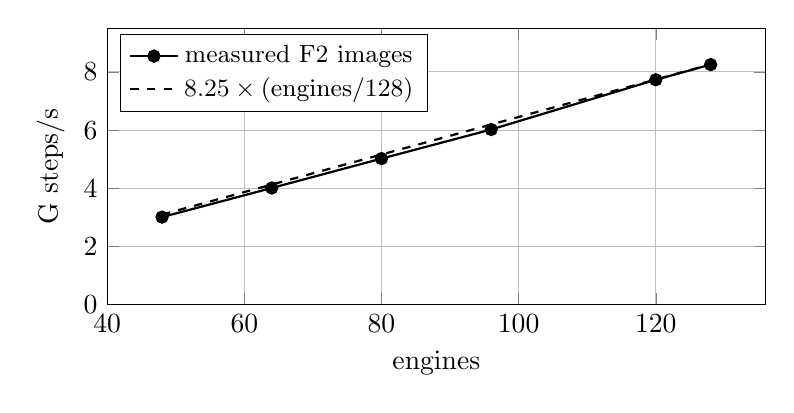
\begin{tikzpicture}
\begin{axis}[
  width=0.82\textwidth,
  height=0.42\textwidth,
  xlabel={engines},
  ylabel={G steps/s},
  xmin=40, xmax=136,
  ymin=0, ymax=9.5,
  grid=major,
  legend style={at={(0.02,0.98)},anchor=north west,font=\small},
]
\addplot[mark=*,thick] coordinates {
  (48,3.01) (64,4.01) (80,5.02) (96,6.02) (120,7.73) (128,8.25)
};
\addlegendentry{measured F2 images}
\addplot[dashed,domain=48:128,thick] {0.0645*x};
\addlegendentry{$8.25\times(\mathrm{engines}/128)$}
\end{axis}
\end{tikzpicture}
\caption{Companion ECC2K-130 FPGA engine on AWS F2. The 128-engine
  image at $333$~MHz is $8.25$~G steps/s. Linear scaling with engine
  count is the prediction of a design that shares nothing between
  engines except the host port. This library's digit-serial core is
  not on this figure: it has no fmax.}
\label{fig:fpga}
\end{figure}

FPGA workers speak the same client contract as the GPUs and write the
same 32-byte records, so a collision between an FPGA trail and a GPU
trail is an ordinary merge.

\section{ECC2K-130 campaign and structural negatives}
\label{sec:campaign}

The live campaign is a $\sigma$-walk, not the $20.08$~B/s table-walk
corpus. Its configuration is \texttt{crypto:ecc2k130/aws/campaign.json}:
\texttt{dpWeight}${}=32$, batch $16$, 256-thread blocks, two blocks/SM,
$385{,}024$ workers ${}=6{,}160{,}384$ logical walks, $1{,}024$
steps/launch, \texttt{maxIters}${}=2^{30}$. Native carry-less
multiplication is what moved the campaign onto CUDA 13.3 and onto
batch 16.\art{crypto:ecc2k130/aws/campaign.json}

\subsection{Cutoff 32, $2^{28.41}$ iterations per point}

An earlier fleet-wide ratio of $7.93\cdot 10^{15}$ checkpointed
iterations against $31.6$~M uploaded points had been quoted as
$2^{27.9}$ iterations per point. Neither counter was clean: the
checkpoint sum multiplied every slot's per-walk base by one campaign
constant, and the point total mixed in the first two slots, which
walked at weight 34. A ratio of a mis-weighted sum to a mixed count
is not a measurement of the running cutoff.

The calibration that replaced it reads, from each live worker, the
client's own two counters --- iterations this run, computed on the
grid the client built itself, and distinguished points over the same
interval. Frozen at 2026-09-17 18:47 UTC, 132 workers
(Table~\ref{tab:cutoff}):\art{crypto:ecc2k130/benchmarks/dp-interval/README.md}

\begin{table}[t]
\centering
\small
\caption{Iterations per distinguished point at cutoff 32. One report
  per $2^{28.41}=3.56\cdot 10^8$ iterations, the same on every family,
  per-worker spread $0.04$ in the exponent.}
\label{tab:cutoff}
\begin{tabular}{@{}lrrrr@{}}
\toprule
family & workers & iterations & points & it/point \\
\midrule
RTX PRO 6000 (g7e) & 38 & $5.606\cdot 10^{15}$ & 15.7~M & $2^{28.41}$ \\
L40S (g6e) & 34 & $2.723\cdot 10^{15}$ & 7.6~M & $2^{28.41}$ \\
RTX PRO 4500 (g7) & 48 & $3.081\cdot 10^{15}$ & 8.6~M & $2^{28.41}$ \\
CPU & 12 & $2.804\cdot 10^{14}$ & 0.79~M & $2^{28.41}$ \\
all & 132 & $1.169\cdot 10^{16}$ & 32.8~M & $\mathbf{2^{28.41}}$ \\
\bottomrule
\end{tabular}
\end{table}

Expected work remains $2^{60.9}=2.15\cdot 10^{18}$ iterations. At
weight 32 the expected corpus is about $2^{32.5}$ records, $0.19$~TB;
about $40$ points/s, $3.4$~M points/day, $0.11$~GB/day per GPU at the
$14.11$~B/s DP34 collection rate of the audited packed
$\sigma$-walk.\art{crypto:ecc2k130/aws/README.md}

\subsection{Certification and the 124~M-point snapshot}

The storage protocol uses checksummed manifests, pinned
worker/replay binaries and lease-fenced checkpoint pointers. Every
walk seed is derived from a 16-bit \texttt{--run-id}; two contributors
who pick different ids never repeat each other's trail. A distinguished
point is a 32-byte record; a collision between any two corpora is
solved by reloading them and replaying both walks. The public
dashboard publishes aggregates only: not point keys, coefficients,
seeds, or database URLs. Checkpointed iteration totals --- not just
point counts --- are the conservative fleet-rate estimator.

The ``$\sim 124$~M points'' figure is a dated storage-recovery
snapshot, not the expected collision corpus. After ingesting
$63{,}351{,}803$ rows the store went from $67.6$~M points to
$124.3$~M, with zero failed or outstanding objects and no
collision.\art{crypto:ecc2k130/aws/README.md, ingest paragraph}
No collision is the expected state: $124$~M points at cutoff 32 is
about $2^{55.3}$ iterations, a fraction of $2^{60.9}$.

\subsection{Structural negatives}

Several alternatives were measured and did not pay. They are listed
because a later thread that rediscovers them should find the
measurement rather than the folklore.

\begin{itemize}[leftmargin=1.2em,itemsep=0.4em]
\item \emph{A $28$~B/s one-addition walk on one GPU.} Below the
  carry-less-unit floor (Section~\ref{sec:floor28}).
\item \emph{The table walk as campaign default.} Measured $16.56$~B/s
  against a pre-declared $17.0$; declined
  (Section~\ref{sec:tablewalk}).
\item \emph{A Modal SKU that beats the RTX~PRO~6000.} Surveyed; none
  did (Table~\ref{tab:survey}).
\item \emph{Bitsliced rewrite as the path to $20$~B/s.} The generated
  bitsliced multiplier's instruction ceiling does not reach it; the
  packed path with \texttt{clmad} is what did.\art{crypto:ecc2k130/THROUGHPUT-CEILING.md}
\item \emph{Index calculus on the Koblitz curve as an ECC2K-130
  solver.} The boundary ledger's best Koblitz row at a 39-bit
  subgroup is $S=58.8$, $300\times$ signed-Frobenius rho
  (Section~\ref{sec:ic-elliptic}). Meet-in-the-middle point
  decomposition at ECC2K-130-like $(m,\ell)$ sits $35$--$51$ bits over
  the per-PDP budget.\art{experiments/pdp-scaling/README.md}
\item \emph{Quoting $2^{27.9}$ as the cutoff-32 interval.} Accounting
  error; replaced by $2^{28.41}$ (Table~\ref{tab:cutoff}).
\end{itemize}

Each is engineering, relabelling, or accounting. None is an advance on
the generic-group floor, which for this problem is still $\sqrt{\pi
r/(2\cdot 262)}$ class-walk steps.

\section{Index calculus over prime fields}
\label{sec:indexcalc}

Index calculus is the algorithm whose exponent is supposed to beat
one half. In $(\ZZ/p\ZZ)^*$ it does, near $56$~bits on this library.
On $E(\FF_p)$ and $E(\FF_{p^3})$ it does not, at any size that fits.
A genus-3/4 Jacobian is the positive control that shows the unit can
register a crossover when one exists.

\subsection{\texorpdfstring{Linear sieve in $(\ZZ/p\ZZ)^*$}{Linear sieve in (Z/pZ)*}}
\label{sec:ic-mult}

The library implements the Coppersmith--Odlyzko--Schroeppel linear
sieve~\cite{cos1986}. With $H=\lceil\sqrt{p}\rceil$ and $J=H^2-p$,
\[
  (H+c_1)(H+c_2) \;=\; J+(c_1+c_2)H+c_1c_2 \pmod{p},
\]
and the right-hand side is $O(C\sqrt{p})$ for $|c_i|\le C$, so it is
$B$-smooth far more often than a random residue. Unknowns are the logs
of the primes up to $B$ and of the $2C+1$ numbers $H+c$. Heuristic
complexity $L_p[1/2,1]$. Random-exponent collection ($L_p[1/2,2]$) is
kept as an independent check of the linear
algebra.\art{src/indexcalc.c}\art{docs/ALGORITHMS.md, ``Index calculus''}

Linear algebra is modulo $p-1=\prod q^e$. For $q\le 2^{24}$ the
factor-base logs are computed directly with Pohlig--Hellman in the
small subgroups. For each larger $q$ the relation matrix is solved
modulo $q$: structured Gaussian elimination, then Lanczos on $A^TDA$
with a random diagonal $D$ (LaMacchia--Odlyzko~\cite{lamacchia1990}),
Hensel-lifted for $e>1$. Every factor-base logarithm is verified
($\zeta^{\log}=q\bmod p$) before it is used. Individual logarithms
are randomised smoothness trials of $h\zeta^e$; at these sizes a few
hundred trial divisions suffice, so there is no descent stage.

Table~\ref{tab:ic-zp} is a re-run of \texttt{ca\_bench ic --threads 4}
on this machine, extended from the published $32$--$56$-bit table
through $60$ and $62$~bits. The $32$--$56$ columns match the published
factor-base and unknown counts; wall-clock differs because the host
differs. The $60$ and $62$-bit rows did not appear in the published
table and are marked as this extension.\art{paper/ic-rerun.txt}\art{docs/BENCHMARKS.md, Index calculus in (Z/pZ)*}

\begin{table}[t]
\centering
\small
\caption{Linear sieve in $(\ZZ/p\ZZ)^*$, safe primes $p=2q+1$, 4
  threads, this machine. ``rho ops'' is $1.3\sqrt{q}$. Rows $60$ and
  $62$ are the extension.}
\label{tab:ic-zp}
\begin{tabular}{@{}rrrrrrrr@{}}
\toprule
bits & fb & unk. & rels & sieve s & LA s & pre s & rho ops \\
\midrule
32 & 53 & 354 & 1\,290 & 0.002 & 0.013 & 0.015 & $4.3\cdot 10^{4}$ \\
40 & 125 & 926 & 1\,919 & 0.001 & 0.043 & 0.045 & $6.8\cdot 10^{5}$ \\
48 & 303 & 2\,504 & 3\,657 & 0.003 & 0.170 & 0.173 & $1.1\cdot 10^{7}$ \\
56 & 669 & 6\,270 & 7\,794 & 0.013 & 0.793 & 0.806 & $1.7\cdot 10^{8}$ \\
60$^*$ & 1\,007 & 10\,008 & 11\,396 & 0.014 & 1.614 & 1.629 & $7.0\cdot 10^{8}$ \\
62$^*$ & 1\,284 & 12\,785 & 14\,675 & 0.014 & 2.697 & 2.712 & $1.4\cdot 10^{9}$ \\
\bottomrule
\end{tabular}\\[0.3em]
{\footnotesize $^*$ extension, this machine; not in the published table.}
\end{table}

The sieve is essentially free; the cost is Lanczos, which grows as
$(\text{unknowns})^2$. At the published $Z_p^*$ rate of $169.4$~Mops/s,
rho at $56$~bits is about $1.0$~s of multiply-equivalents against
$0.81$~s of index-calculus precomputation on this host, confirming the
published crossover near $56$~bits. At $60$ and $62$~bits the same
conversion gives about $4.1$~s and $8.3$~s of rho against $1.63$~s and
$2.71$~s of sieve-plus-Lanczos: the gap widens, as $L_p[1/2]$ against
$N^{1/2}$ says it should. Individual logarithms remain negligible
($147$--$1{,}310$ trial divisions).

This is an $L_p[1/2,1]$ implementation. The state of the art above
roughly $100$~bits is the number field sieve ($L_p[1/3]$); NFS is out
of scope for a 64-bit toolkit.

\subsection{Elliptic curves: the negative, phase by phase}
\label{sec:ic-elliptic}

For elliptic curves over prime fields no index calculus is known that
beats rho at any cryptographic size~\cite{semaev2004,gaudry2009,diem2011}.
The sibling's boundary ledger puts three regimes --- a generic
prime-field curve, a random binary curve, and a Koblitz curve --- on
the same axis, every phase charged, every logarithm
verified.\art{crypto:research/notes/index-calculus/RESEARCH_IC_BOUNDARY_LEDGER.md}

Headline cells, full pipeline:

\begin{center}
\small
\begin{tabular}{@{}llrrr@{}}
\toprule
regime & best variant & $S$ & vs rho & vs floor \\
\midrule
prime, $23.4$-bit subgroup & MITM $m=3$ & $56.8$ & $14.5\times$ & $64.1\times$ \\
random binary, $24.4$-bit & MITM $m=3$ & $206$ & $89\times$ & $232\times$ \\
Koblitz, $39$-bit subgroup & orbit-column MITM & $58.8$ & $300\times$ & $425\times$ \\
\bottomrule
\end{tabular}
\end{center}

Matched rho on those instances: $S=3.93$ (prime), $S=2.31$ (binary),
signed-Frobenius $S=0.20$ (Koblitz). Fitted full-pipeline exponents:
prime MITM $m=3$ at $0.60$; binary MITM $m=3$ at $0.62$; Koblitz
signed-orbit MITM at $0.54$ overall, or $0.51$ on cofactor-${}\le 4$
rungs. All are above one half. No cell is below matched rho.

Oracle rounds that price only the decomposition of one residual are
stage diagnostics. They do not enter the $S$ column and are not
reported as speedups.

\subsection{\texorpdfstring{$E(\FF_{p^3})$ residual walks}{E(F_p^3) residual walks}}
\label{sec:ic-cubic}

The residual-walk note is the worked negative
(Section~\ref{sec:method-residual}). The prime-field route loses
because it has no proper additive subspace; the $S_3$ oracle pays per
base element. On $E(\FF_{p^3})$ a factor base that is an
$\FF_p$-subspace lets a residual be a walk, and the counting floor of
§9.6 applies.

A MITM triple oracle at $p=271$ to $2083$ ($n=2^{24.2}$ to $2^{33.1}$)
measures $S=1{,}224\to 3{,}805$, i.e.\ $1{,}057\times\to 2{,}240\times$
rho, fitted total exponent $0.69$ against a prediction of $2/3$.
Building a base-independent $S_4$ solve left an initial $C_3$ of
$4.7$--$4.9$ million $\FF_p$-multiplications per residual; the
relation-only crossover extrapolated to $2^{111}$. Engineering in
§§11.5--11.6 reduced $C_3$ to $879{,}000$, a $5.5\times$ improvement,
and the relation-only crossover became $2^{96}$. That $2^{96}$ is a
stage diagnostic.

Section~11.7 restores full accounting. Sequential Wiedemann over
$\ZZ/n\ZZ$, multiplications modulo $n\approx p^3$ charged as $9$
$\FF_p$ multiplications, every run correct
(Table~\ref{tab:gaudry-la}):\art{crypto:research/notes/index-calculus/RESEARCH_RESIDUAL_WALKS.md, §11.7}

\begin{table}[t]
\centering
\small
\caption{$E(\FF_{p^3})$ residual walks, full pipeline. $S$ includes
  relations, filtering and linear algebra. Every run recovered the
  planted logarithm.}
\label{tab:gaudry-la}
\begin{tabular}{@{}rrlrrr@{}}
\toprule
$p$ & $n$ & variant & $S$ & $S/$rho & LA share \\
\midrule
271 & $2^{24.2}$ & dense & 2\,696 & $2{,}328\times$ & $0.05\%$ \\
271 & $2^{24.2}$ & Wiedemann & 2\,830 & $2{,}443\times$ & $0.19\%$ \\
271 & $2^{24.2}$ & + large primes & 4\,634 & $4{,}000\times$ & $0.02\%$ \\
523 & $2^{27.1}$ & dense & 1\,989 & $1{,}680\times$ & $0.10\%$ \\
1\,039 & $2^{30.1}$ & dense & 1\,236 & $903\times$ & $0.31\%$ \\
2\,083 & $2^{33.1}$ & dense & 898 & $528\times$ & $1.22\%$ \\
2\,083 & $2^{33.1}$ & Wiedemann & 974 & $574\times$ & $1.61\%$ \\
2\,083 & $2^{33.1}$ & + large primes & 3\,378 & $1{,}989\times$ & $0.03\%$ \\
\bottomrule
\end{tabular}
\end{table}

Fitted exponents over the four sizes: dense total $n^{0.32}$,
Wiedemann linear algebra $n^{0.68}$ ($N^{2.00}$ in the number of
unknowns), double large primes total $n^{0.44}$ near $4/9$. Relations
cost $n^{1/3}$ and the linear algebra $n^{0.68}$ at best, so $S$ falls
as $n^{-1/6}$ while the linear-algebra term rises as $n^{+0.18}$.
Extrapolating the two measured terms, $S$ bottoms out at $\approx 265$
around $n\approx 2^{50}$ --- still $\approx 200\times$ rho --- and
rises after. Double large primes cost $1{,}989\times$ rho at $33$
bits; the extrapolated whole-method crossover is past $2^{230}$. Both
crossovers are extrapolations and are marked as such.

\subsection{Joux--Vitse pair-only}

Decompositions into $k-1$ points~\cite{jouxvitse2013} cut the
per-residual Groebner cost dramatically and grow the residual count.
Table~\ref{tab:paironly} is §11.9 of the residual-walk
note.\art{crypto:research/notes/index-calculus/RESEARCH_RESIDUAL_WALKS.md, §11.9}

\begin{table}[t]
\centering
\small
\caption{Joux--Vitse pair-only versus the $S_4$ hybrid, full
  pipeline. At $33$ bits the per-residual constant has improved about
  $580\times$ while residual growth wins: relabelling.}
\label{tab:paironly}
\begin{tabular}{@{}rrrrr@{}}
\toprule
$p$ & $n$ & $S$ & $S/$rho & residuals \\
\midrule
271 & $2^{24.2}$ & 427 & $534\times$ & 1\,513 \\
523 & $2^{27.1}$ & 1\,331 & $951\times$ & 1\,557 \\
1\,039 & $2^{30.1}$ & 1\,655 & $1{,}273\times$ & 1\,810 \\
2\,083 & $2^{33.1}$ & 1\,659 & $1{,}037\times$ & 1\,857 \\
\bottomrule
\end{tabular}
\end{table}

Residuals fit $n^{0.67}$, total $n^{0.72}$, so $S$ grows as
$n^{+0.22}$. Pair-only is the best local cell below roughly
$n=2^{28.5}$; at $33$ bits it is relabelling. Rho still costs
$S\approx 1.3$ and the best row in the table is $427$.

\subsection{Genus 3/4 Jacobian, the positive control}
\label{sec:ic-hyper}

Adleman--DeMarrais--Huang / Enge index calculus on a hyperelliptic
Jacobian of genus $g$ has predicted cost $O(g^2 q^{2-2/g+\varepsilon})$
against rho's $O(\sqrt{q^g})=O(q^{g/2})$. The ratio
$S_{\mathrm{IC}}/S_{\rho}$ should therefore fall as $N^{1/g-1/2}$:
flat at genus $2$, slope $-1/6$ at genus $3$, slope $-1/4$ at genus
$4$. Figure~\ref{fig:hyper} and Table~\ref{tab:hyper} are the sibling's
round-four/five measurements, every row a verified
$k$.\art{crypto:research/notes/index-calculus/RESEARCH_HYPERELLIPTIC_IC_RHO.md}

\begin{table}[t]
\centering
\small
\caption{Hyperelliptic index calculus versus distinguished-point rho.
  ``corr'' renormalises rho's walk to $\sqrt{\pi/2}$. Toy-sized,
  $p\le 251$.}
\label{tab:hyper}
\begin{tabular}{@{}rrrrrr@{}}
\toprule
$g$ & $p$ & $N$ & $S_{\mathrm{IC}}$ & $S_{\rho}$ & corr. ratio \\
\midrule
3 & 61 & 124\,459 & 1.51 & 2.30 & 0.73 \\
3 & 101 & 364\,747 & 1.12 & 1.90 & 0.64 \\
3 & 151 & 1\,180\,351 & 0.79 & 1.98 & 0.52 \\
3 & 211 & 4\,620\,611 & 0.53 & 1.96 & 0.38 \\
4 & 31 & 239\,753 & 1.77 & 1.90 & 0.95 \\
4 & 41 & 333\,041 & 1.41 & 1.86 & 0.80 \\
4 & 61 & 16\,790\,591 & 0.28 & 2.17 & \textbf{0.21} \\
\bottomrule
\end{tabular}
\end{table}

Fitted slopes against $\log_2 N$: genus $2$ at $-0.027$ ($R^2=0.24$,
no trend, prediction $0$); genus $3$ at $-0.154$ ($R^2=0.98$,
prediction $-1/6$); genus $4$ at $-0.275$ ($R^2=0.96$, prediction
$-1/4$). The law holds. Genus $3$ at $p=61$ and $p=101$ already sits
at $S_{\mathrm{IC}}/S_{\rho}=0.66$ and $0.61$ in the raw column; genus
$4$ at $p=61$, $N\approx 2^{24}$, reaches $0.21$ after the walk
renormalisation. That is the crossover this paper's unit was built to
see, and it appears on Jacobians, not on elliptic curves.

\begin{figure}[t]
\centering
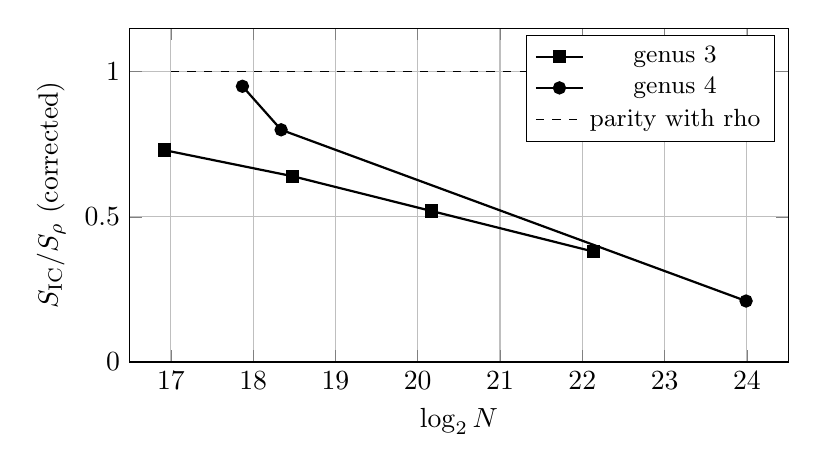
\begin{tikzpicture}
\begin{axis}[
  width=0.82\textwidth,
  height=0.48\textwidth,
  xlabel={$\log_2 N$},
  ylabel={$S_{\mathrm{IC}}/S_{\rho}$ (corrected)},
  xmin=16.5, xmax=24.5,
  ymin=0, ymax=1.15,
  grid=major,
  legend style={at={(0.98,0.98)},anchor=north east,font=\small},
]
\addplot[mark=square*,thick] coordinates {
  (16.92,0.73) (18.48,0.64) (20.17,0.52) (22.14,0.38)
};
\addlegendentry{genus 3}
\addplot[mark=*,thick] coordinates {
  (17.87,0.95) (18.34,0.80) (23.99,0.21)
};
\addlegendentry{genus 4}
\addplot[dashed,domain=17:24] {1};
\addlegendentry{parity with rho}
\end{axis}
\end{tikzpicture}
\caption{Hyperelliptic positive control. The ratio to distinguished-point
  rho falls at genus $3$ and genus $4$ with the predicted slopes.
  No measured end-to-end elliptic variant of Sections~\ref{sec:ic-elliptic}
  and~\ref{sec:ic-cubic} has crossed this line.}
\label{fig:hyper}
\end{figure}

\section{Related work}
\label{sec:related}

Pollard's rho method~\cite{pollard1978} and Shanks' baby-step
giant-step~\cite{shanks1971} are the generic algorithms. Teske's
$r$-adding walk~\cite{teske2001} is the mixing rule this library uses;
van Oorschot--Wiener~\cite{vanoorschot1999} is the parallelisation;
Bernstein--Lange--Schwabe~\cite{bls2011} is the correct use of the
negation map. Two grumpy giants and a baby~\cite{bernsteinlange2012grumpy}
and free precomputation~\cite{bernsteinlange2012small,bernsteinlange2013}
are priced as neighbours, not as replacements. Wiener--Zuccherato and
Duursma--Gaudry--Morain~\cite{wienerzuccherato1998,duursma1999} folded
rho by the automorphism group; GLV~\cite{glv2001} is the constructive
counterpart that this library applies automatically on $j=0$ and
$j=1728$. Cheon~\cite{cheon2006,cheon2010} is a different problem ---
DLP with auxiliary inputs --- and is labelled as such.

The linear sieve~\cite{cos1986} and Lanczos over finite
fields~\cite{lamacchia1990} are the $(\ZZ/p\ZZ)^*$ solver. Semaev
summation polynomials~\cite{semaev2004}, Gaudry's index calculus for
abelian varieties of small dimension~\cite{gaudry2009}, Diem's analysis
of the elliptic discrete logarithm~\cite{diem2011}, and Joux--Vitse
pair decompositions~\cite{jouxvitse2013} are the elliptic side. The
contribution here is not a new algorithm; it is a measurement in one
unit, with every phase priced, against a floor that cannot be tuned
away.

ECC2K-130 is Bailey et al.~\cite{bailey2009}, building on Harley's
ECC2K-95~\cite{harley1998} and Certicom's challenge
list~\cite{certicom1997}. Itoh--Tsujii
inversion~\cite{itoh1988} and Montgomery's simultaneous
inversion~\cite{montgomery1987} are the two inversion tricks the
designs spend most of their area and most of their GPU time on. The
FPGA and GPU numbers in Sections~\ref{sec:ecc2k-gpu} and~\ref{sec:ecc2k-fpga}
are this programme's, cited to their artefacts; they are not a claim
to have broken the challenge.

The reporting rule --- boundary, one unit, four classes, phases priced
separately, extrapolations marked --- is the sibling study library's
standing convention, written to stop a thread from spending weeks
improving a headline constant while the ratio to the floor stays
flat. Wesolowski's supersingular-isogeny result in time
$p^{1/3+o(1)}$ is the target-result profile that convention is aimed
at: exponent-first, heuristics numbered, phases booked as
per-attempt-cost times inverse success probability. This paper is a
measurement paper, not that theorem; the profile is named so the
negative elliptic result is read as a finished thread, not as a
pause.


\section{Conclusion}
\label{sec:conclusion}

Three statements survive the accounting.

First, Pollard rho on this library is a measured constant, not a slogan:
$S \approx 1.2$--$1.8$ across 24--40~bits, with the negation map, Teske's
$r$-adding walk, Bernstein--Lange--Schwabe cycle handling, and one
inversion per 256 additions all inside the count. Independent
implementations in the companion recover the same constant (rho $S=0.85$
against BSGS $S=1.07$; a Frobenius-class walk at $0.94\times$ and
$1.32\times$ of its own prediction). Nothing here is an advance on the
generic-group floor.

Second, ECC2K-130 is an arithmetic problem at a known exponent. The
GPU ledger from a bitsliced control at $0.85$~B/s to a packed walk at
$14.64$~B/s is engineering against a carry-less-unit floor that rules
out $28$~B/s on one GPU. A table walk measured $16.56$~B/s against a
pre-declared $17.0$ and was declined. A digit-serial FPGA core in this
library takes $362$ cycles/step at $7{,}941$ LUT4; a companion engine
on an AWS F2 holds $8.25$~G~steps/s. The live fleet walks at cutoff
$32$, one report per $2^{28.41}$ iterations, with about $124$~M points
and no collision. Structural alternatives (index calculus on the
Koblitz curve, a $28$~B/s one-addition walk, a SKU that beats the
RTX~PRO~6000) were measured and did not pay.

Third, index calculus over $(\ZZ/p\ZZ)^*$ crosses rho near $56$~bits
and pulls away. Index calculus on $E(\FF_p)$ and $E(\FF_{p^3})$ does
not: at the sizes that fit, every end-to-end elliptic variant costs
between $14.5\times$ and $4{,}000\times$ matched rho, and the
asymptotically better $E(\FF_{p^3})$ hybrid bottoms near $200\times$
rho around $2^{50}$ and rises. The genus-3/4 Jacobian is the positive
control that shows the unit can register a crossover when one exists.

The constant in front of $\sqrt{n}$ is the right quantity. On the
curves that matter it has not yet fallen below one.

\appendix
\section{Reproduction commands}
\label{app:repro}

Commands below are from the two repository roots. They reproduce the
tables, not the GPU or F2 measurements: those need the named card or
image. Every answer the library returns is checked against a planted
secret inside the tool; a row that is not \texttt{ok} is not a result.

\subsection{This library}

\begin{verbatim}
cmake -S . -B build -DCMAKE_BUILD_TYPE=Release
cmake --build build -j
ctest --test-dir build

# Table 1, Table 2 (S and fitted exponents)
./build/ca_bench generic --threads 4
./build/ca_bench complexity --bits 20,24,28,32,36 --reps 5
./build/ca_bench ops
./build/ca_bench interval
./build/ca_bench precomp --threads 1
./build/ca_bench glv
./build/ca_bench cheon
./build/ca_bench gpu          # host emulator; no device required

# Table 5, including the 60/62-bit extension
./build/ca_bench ic --bits 32,40,48,56,60,62 --threads 4

# Golden model and FPGA vectors (no vendor tools)
make -C fpga test            # or: fpga/scripts/run_sim.sh
make -C ecc2k130             # 1,904 checks, no CUDA
\end{verbatim}

\noindent Sources: \texttt{docs/BENCHMARKS.md},
\texttt{docs/ALGORITHMS.md}, \texttt{fpga/README.md},
\texttt{ecc2k130/README.md}.

\subsection{Sibling study library}

\begin{verbatim}
# Rho / BSGS walk-check (CPU emulation of the kernels)
make -C gpu/ecc test
make -C gpu/ecc2k test

# Boundary ledger (the three-regime elliptic table)
cargo build --release --bin ic
./target/release/ic boundary --oracles --out /tmp/ledger.json

# Hyperelliptic positive control
cargo run --release --example hyperelliptic_ic_vs_rho
python3 scripts/hyperelliptic_exponent_fit.py

# Residual-walk note: the commands are in
# research/notes/index-calculus/RESEARCH_RESIDUAL_WALKS.md §11
# Frozen scoreboard (read, do not recompute):
# docs/index-calculus-scoreboard.html
\end{verbatim}

GPU throughput rows need an RTX~PRO~6000 (or the named Modal SKU) and
CUDA ${}\ge 13.3$ for \texttt{clmad}. The F2 row needs the 128-engine
image in \texttt{hdl/ecc2k130/aws/}. The campaign counters are frozen
in \texttt{ecc2k130/benchmarks/dp-interval/raw/}.

\subsection{This paper}

\begin{verbatim}
cd paper
make            # ecdlp.pdf
make check      # unresolved refs, overfull boxes, page count
make arxiv      # arxiv-submission.tar.gz
make eprint     # eprint-submission.zip
\end{verbatim}

Restore authors with \texttt{cp AUTHORS.example AUTHORS}, edit, and
\texttt{make deanonymize}.


\bibliographystyle{plainnat}
\bibliography{ecdlp}

\end{document}
